%
% Copyright (c) 2006-2007 XenSource, Inc.
%
% All rights reserved.
%
% Authors: Ewan Mellor, Richard Sharp, Dave Scott, Jon Harrop.
%

\documentclass{report}

\usepackage{geometry}
\usepackage{layout}
\geometry{
  left=2.0cm,
  right=2.5cm,
  top=3.5cm,
  bottom=3cm
}
\usepackage{graphics}
\usepackage{longtable}
\usepackage{fancyhdr}

\setlength\parindent{0pt}

%% Parameters for coversheet:
%
% Copyright (c) 2006-2007 XenSource, Inc.
%
% All rights reserved.
%
% Authors: Ewan Mellor, Richard Sharp, Dave Scott, Jon Harrop.
%

%% Document title
\newcommand{\doctitle}{Xen Management API}

\newcommand{\coversheetlogo}{xen.eps}

%% Document date
\newcommand{\datestring}{5th April 2007}

\newcommand{\releasestatement}{Candidate for Release\\Comments are welcome!}

%% Document revision
\newcommand{\revstring}{API Revision 0.9.0}

%% Document authors
\newcommand{\docauthors}{
Ewan Mellor: & {\tt ewan@xensource.com} \\
Richard Sharp: & {\tt richard.sharp@xensource.com} \\
David Scott: & {\tt david.scott@xensource.com}}
\newcommand{\legalnotice}{Copyright \copyright{} 2006-2007 XenSource, Inc.\\ \\
Permission is granted to copy, distribute and/or modify this document under
the terms of the GNU Free Documentation License, Version 1.2 or any later
version published by the Free Software Foundation; with no Invariant Sections,
no Front-Cover Texts and no Back-Cover Texts.  A copy of the license is
included in the section entitled "GNU Free Documentation License".
}


\begin{document}

% The coversheet itself
%
% Copyright (c) 2006-2007 XenSource, Inc.
%
% All rights reserved.
%
% Authors: Ewan Mellor, Richard Sharp, Dave Scott, Jon Harrop.
%

\pagestyle{empty}

\doctitle{} \hfill \revstring{}

\vspace{1cm}

\begin{center}
\resizebox{8cm}{!}{\includegraphics{\coversheetlogo}}

\vspace{2cm}

\begin{Huge}
  \doctitle{}
\end{Huge}

\vspace{1cm}
\begin{Large}
\revstring{}\\
\releasestatement{}

\vspace{1cm}
\begin{tabular}{rl}
\docauthors{}
\end{tabular}
\end{Large}
\end{center}
\vspace{.5cm}

\vfill

\noindent
\legalnotice{}

\newpage
\pagestyle{fancy}

% ... and off we go!

\chapter{Introduction}

This document contains a description of the Xen Management API---an interface for
remotely configuring and controlling virtualised guests running on a
Xen-enabled host. 

%
% Copyright (c) 2006-2007 XenSource, Inc.
%
% All rights reserved.
%
% Authors: Ewan Mellor, Richard Sharp, Dave Scott, Jon Harrop.
%

The API is presented here as a set of Remote Procedure Calls, with a wire
format based upon XML-RPC. No specific language bindings are prescribed,
although examples will be given in the python programming language.
 
Although we adopt some terminology from object-oriented programming, 
future client language bindings may or may not be object oriented.
The API reference uses the terminology {\em classes\/} and {\em objects\/}.
For our purposes a {\em class\/} is simply a hierarchical namespace;
an {\em object\/} is an instance of a class with its fields set to
specific values. Objects are persistent and exist on the server-side.
Clients may obtain opaque references to these server-side objects and then
access their fields via get/set RPCs.

%In each class there is a $\mathit{uid}$ field that assigns an indentifier
%to each object. This $\mathit{uid}$ serves as an object reference
%on both client- and server-side, and is often included as an argument in
%RPC messages.

For each class we specify a list of
fields along with their {\em types\/} and {\em qualifiers\/}.  A
qualifier is one of:
\begin{itemize}
  \item $\mathit{RO}_\mathit{run}$: the field is Read
Only. Furthermore, its value is automatically computed at runtime.
For example: current CPU load and disk IO throughput.
  \item $\mathit{RO}_\mathit{ins}$: the field must be manually set
when a new object is created, but is then Read Only for
the duration of the object's life.
For example, the maximum memory addressable by a guest is set 
before the guest boots.
  \item $\mathit{RW}$: the field is Read/Write. For example, the name
of a VM.
\end{itemize}

A full list of types is given in Chapter~\ref{api-reference}. However,
there are three types that require explicit mention:
\begin{itemize}
  \item $t~\mathit{Ref}$: signifies a reference to an object
of type $t$.
  \item $t~\mathit{Set}$: signifies a set containing
values of type $t$.
  \item $(t_1, t_2)~\mathit{Map}$: signifies a mapping from values of
type $t_1$ to values of type $t_2$.
\end{itemize}

Note that there are a number of cases where {\em Ref}s are {\em doubly
linked\/}---e.g.\ a VM has a field called {\tt VIFs} of type
$(\mathit{VIF}~\mathit{Ref})~\mathit{Set}$; this field lists
the network interfaces attached to a particular VM. Similarly, the VIF
class has a field called {\tt VM} of type $(\mathit{VM}~{\mathit
Ref})$ which references the VM to which the interface is connected.
These two fields are {\em bound together\/}, in the sense that
creating a new VIF causes the {\tt VIFs} field of the corresponding
VM object to be updated automatically.

The API reference explicitly lists the fields that are
bound together in this way. It also contains a diagram that shows
relationships between classes. In this diagram an edge signifies the
existance of a pair of fields that are bound together, using standard
crows-foot notation to signify the type of relationship (e.g.\
one-many, many-many).

\section{RPCs associated with fields}

Each field, {\tt f}, has an RPC accessor associated with it
that returns {\tt f}'s value:
\begin{itemize}
\item ``{\tt get\_f(Ref x)}'': takes a
{\tt Ref} that refers to an object and returns the value of {\tt f}.
\end{itemize}

Each field, {\tt f}, with attribute
{\em RW} and whose outermost type is {\em Set\/} has the following
additional RPCs associated with it:
\begin{itemize}
\item an ``{\tt add\_to\_f(Ref x, v)}'' RPC adds a new element v to the set\footnote{
%
Since sets cannot contain duplicate values this operation has no action in the case
that {\tt v} was already in the set.
%
};
\item a ``{\tt remove\_from\_f(Ref x, v)}'' RPC removes element {\tt v} from the set;
\end{itemize}

Each field, {\tt f}, with attribute
{\em RW} and whose outermost type is {\em Map\/} has the following
additional RPCs associated with it:
\begin{itemize}
\item an ``{\tt add\_to\_f(Ref x, k, v)}'' RPC adds new pair {\tt (k, v)}
to the mapping stored in {\tt f} in object {\tt x}. Adding a new pair for duplicate
key, {\tt k}, overwrites any previous mapping for {\tt k}.
\item a ``{\tt remove\_from\_f(Ref x, k)}'' RPC removes the pair with key {\tt k}
from the mapping stored in {\tt f} in object {\tt x}.
\end{itemize}

Each field whose outermost type is neither {\em Set\/} nor {\em Map\/}, 
but whose attribute is {\em RW} has an RPC acessor associated with it
that sets its value:
\begin{itemize}
\item For {\em RW\/} ({\em R\/}ead/{\em
W\/}rite), a ``{\tt set\_f(Ref x, v)}'' RPC function is also provided.
This sets field {\tt f} on object {\tt x} to value {\tt v}.
\end{itemize}

\section{RPCs associated with classes}

\begin{itemize}
\item Each class has a {\em constructor\/} RPC named ``{\tt create}'' that
takes as parameters all fields marked {\em RW\/} and
$\mathit{RO}_\mathit{ins}$. The result of this RPC is that a new {\em
persistent\/} object is created on the server-side with the specified field
values.

\item Each class has a {\tt get\_by\_uuid(uuid)} RPC that returns the object
of that class that has the specified {\tt uuid}.

\item Each class that has a {\tt name\_label} field has a
``{\tt get\_by\_name\_label(name)}'' RPC that returns a set of objects of that
class that have the specified {\tt label}.

\item Each class has a ``{\tt destroy(Ref x)}'' RPC that explicitly deletes
the persistent object specified by {\tt x} from the system.  This is a
non-cascading delete -- if the object being removed is referenced by another
object then the {\tt destroy} call will fail.

\end{itemize}

\subsection{Additional RPCs}

As well as the RPCs enumerated above, some classes have additional RPCs
associated with them. For example, the {\tt VM} class has RPCs for cloning,
suspending, starting etc. Such additional RPCs are described explicitly
in the API reference.


%
% Copyright (c) 2006-2007 XenSource, Inc.
%
% All rights reserved.
%
% Authors: Ewan Mellor, Richard Sharp, Dave Scott, Jon Harrop.
%

\section{Wire Protocol for Remote API Calls}

API calls are sent over a network to a Xen-enabled host using
the XML-RPC protocol. In this Section we describe how the
higher-level types used in our API Reference are mapped to
primitive XML-RPC types.

In our API Reference we specify the signatures of API functions in the following
style:
\begin{verbatim}
    (ref_vm Set)   VM.get_all()
\end{verbatim}
This specifies that the function with name {\tt VM.get\_all} takes
no parameters and returns a Set of {\tt ref\_vm}s.
These types are mapped onto XML-RPC types in a straight-forward manner:
\begin{itemize}
  \item Floats, Bools, DateTimes and Strings map directly to the XML-RPC {\tt
  double}, {\tt boolean}, {\tt dateTime.iso8601}, and {\tt string} elements.

  \item all ``{\tt ref\_}'' types are opaque references, encoded as the
  XML-RPC's {\tt String} type. Users of the API should not make assumptions
  about the concrete form of these strings and should not expect them to
  remain valid after the client's session with the server has terminated.

  \item fields named ``{\tt uuid}'' of type ``{\tt String}'' are mapped to
  the XML-RPC {\tt String} type. The string itself is the OSF
  DCE UUID presentation format (as output by {\tt uuidgen}, etc).

  \item ints are all assumed to be 64-bit in our API and are encoded as a
  string of decimal digits (rather than using XML-RPC's built-in 32-bit {\tt
  i4} type).

  \item values of enum types are encoded as strings. For example, a value of
  {\tt destroy} of type {\tt on\_normal\_exit}, would be conveyed as:
  \begin{verbatim}
    <value><string>destroy</string></value>
  \end{verbatim}

  \item for all our types, {\tt t}, our type {\tt t Set} simply maps to
  XML-RPC's {\tt Array} type, so for example a value of type {\tt String
  Set} would be transmitted like this:

  \begin{verbatim}
<array>
  <data>
    <value><string>CX8</string></value>
    <value><string>PSE36</string></value>
    <value><string>FPU</string></value>
  </data>
</array> 
  \end{verbatim}

  \item for types {\tt k} and {\tt v}, our type {\tt (k, v) Map} maps onto an
  XML-RPC struct, with the key as the name of the struct.  Note that the {\tt
  (k, v) Map} type is only valid when {\tt k} is a {\tt String}, {\tt Ref}, or
  {\tt Int}, and in each case the keys of the maps are stringified as
  above. For example, the {\tt (String, double) Map} containing a the mappings
  Mike $\rightarrow$ 2.3 and John $\rightarrow$ 1.2 would be represented as:

  \begin{verbatim}
<value>
  <struct>
    <member>
      <name>Mike</name>
      <value><double>2.3</double></value>
    </member>
    <member>
      <name>John</name>
      <value><double>1.2</double></value>
    </member>
  </struct>
</value>
  \end{verbatim}

  \item our {\tt Void} type is transmitted as an empty string.

\end{itemize}

\subsection{Note on References vs UUIDs}

References are opaque types --- encoded as XML-RPC strings on the wire --- understood
only by the particular server which generated them. Servers are free to choose
any concrete representation they find convenient; clients should not make any 
assumptions or attempt to parse the string contents. References are not guaranteed
to be permanent identifiers for objects; clients should not assume that references 
generated during one session are valid for any future session. References do not
allow objects to be compared for equality. Two references to the same object are
not guaranteed to be textually identical.

UUIDs are intended to be permanent names for objects. They are
guaranteed to be in the OSF DCE UUID presentation format (as output by {\tt uuidgen}.
Clients may store UUIDs on disk and use them to lookup objects in subsequent sessions
with the server. Clients may also test equality on objects by comparing UUID strings.

The API provides mechanisms
for translating between UUIDs and opaque references. Each class that contains a UUID
field provides:
\begin{itemize}
\item  A ``{\tt get\_by\_uuid}'' method that takes a UUID, $u$, and returns an opaque reference
to the server-side object that has UUID=$u$; 
\item A {\tt get\_uuid} function (a regular ``field getter'' RPC) that takes an opaque reference,
$r$, and returns the UUID of the server-side object that is referenced by $r$.
\end{itemize}

\subsection{Return Values/Status Codes}
\label{synchronous-result}

The return value of an RPC call is an XML-RPC {\tt Struct}.

\begin{itemize}
\item The first element of the struct is named {\tt Status}; it
contains a string value indicating whether the result of the call was
a ``{\tt Success}'' or a ``{\tt Failure}''.
\end{itemize}

If {\tt Status} was set to {\tt Success} then the Struct contains a second
element named {\tt Value}:
\begin{itemize}
\item The element of the struct named {\tt Value} contains the function's return value.
\end{itemize}

In the case where {\tt Status} is set to {\tt Failure} then
the struct contains a second element named {\tt ErrorDescription}:
\begin{itemize}
\item The element of the struct named {\tt ErrorDescription} contains
an array of string values. The first element of the array is an error code;
the remainder of the array are strings representing error parameters relating
to that code.
\end{itemize}

For example, an XML-RPC return value from the {\tt host.get\_resident\_VMs}
function above
may look like this:
\begin{verbatim}
    <struct>
       <member>
         <name>Status</name>
         <value>Success</value>
       </member>
       <member>
          <name>Value</name>
          <value>
            <array>
               <data>
                 <value>81547a35-205c-a551-c577-00b982c5fe00</value>
                 <value>61c85a22-05da-b8a2-2e55-06b0847da503</value>
                 <value>1d401ec4-3c17-35a6-fc79-cee6bd9811fe</value>
               </data>
            </array>
         </value>
       </member>
    </struct>
\end{verbatim}

\section{Making XML-RPC Calls}

\subsection{Transport Layer}

The following transport layers are currently supported:
\begin{itemize}
\item HTTP/S for remote administration
\item HTTP over Unix domain sockets for local administration
\end{itemize}

\subsection{Session Layer}

The XML-RPC interface is session-based; before you can make arbitrary RPC calls
you must login and initiate a session. For example:
\begin{verbatim}
   session_id    session.login_with_password(string uname, string pwd, string version, string originator)
\end{verbatim}
Where {\tt uname} and {\tt password} refer to your username and password
while {\tt version} and {\tt originator} are optional and refer to the api version and client name 
respectively, as defined by the Xen administrator.
(The {\tt version} is ignored at present though. A client that doesn't want to specify it can 
send uname, pwd, '', originator)
The {\tt session\_id} returned by {\tt session.login\_with\_password} is passed
to subequent RPC calls as an authentication token.

A session can be terminated with the {\tt session.logout} function:
\begin{verbatim}
   void          session.logout(session_id session)
\end{verbatim}

\subsection{Synchronous and Asynchronous invocation}

Each method call (apart from methods on ``Session'' and ``Task'' objects 
and ``getters'' and ``setters'' derived from fields)
can be made either synchronously or asynchronously.
A synchronous RPC call blocks until the
return value is received; the return value of a synchronous RPC call is
exactly as specified in Section~\ref{synchronous-result}.

Only synchronous API calls are listed explicitly in this document. 
All asynchronous versions are in the special {\tt Async} namespace.
For example, synchronous call {\tt VM.clone(...)}
(described in Chapter~\ref{api-reference})
has an asynchronous counterpart, {\tt
Async.VM.clone(...)}, that is non-blocking.

Instead of returning its result directly, an asynchronous RPC call
returns a {\tt task-id}; this identifier is subsequently used
to track the status of a running asynchronous RPC. Note that an asychronous
call may fail immediately, before a {\tt task-id} has even been created---to
represent this eventuality, the returned {\tt task-id}
is wrapped in an XML-RPC struct with a {\tt Status}, {\tt ErrorDescription} and
{\tt Value} fields, exactly as specified in Section~\ref{synchronous-result}.

The {\tt task-id} is provided in the {\tt Value} field if {\tt Status} is set to
{\tt Success}.

The RPC call
\begin{verbatim}
    (ref_task Set)   Task.get_all(session_id s)
\end{verbatim} 
returns a set of all task IDs known to the system. The status (including any
returned result and error codes) of these tasks
can then be queried by accessing the fields of the Task object in the usual way. 
Note that, in order to get a consistent snapshot of a task's state, it is advisable to call the ``get\_record'' function.

\section{Example interactive session}

This section describes how an interactive session might look, using the python
XML-RPC client library. 

First, initialise python and import the library {\tt xmlrpclib}:

\begin{verbatim}
\$ python2.4
...
>>> import xmlrpclib
\end{verbatim}

Create a python object referencing the remote server:

\begin{verbatim}
>>> xen = xmlrpclib.Server("https://localhost:443")
\end{verbatim}

Acquire a session reference by logging in with a username and password
(error-handling ommitted for brevity; the session reference is returned under the
key {\tt 'Value'} in the resulting dictionary)

\begin{verbatim}
>>> session = xen.session.login_with_password("user", "passwd", "version", "originator")['Value']
\end{verbatim}

When serialised, this call looks like the following:

\begin{verbatim}
<?xml version='1.0'?>
<methodCall>
  <methodName>session.login_with_password</methodName>
  <params>
    <param>
      <value><string>user</string></value>
    </param>
    <param>
      <value><string>passwd</string></value>
    </param>
    <param>
      <value><string>version</string></value>
    </param>
    <param>
      <value><string>originator</string></value>
    </param>
  </params>
</methodCall>
\end{verbatim}

Next, the user may acquire a list of all the VMs known to the system: (Note the
call takes the session reference as the only parameter)

\begin{verbatim}
>>> all_vms = xen.VM.get_all(session)['Value']
>>> all_vms
['OpaqueRef:1', 'OpaqueRef:2', 'OpaqueRef:3', 'OpaqueRef:4' ]
\end{verbatim}

The VM references here have the form {\tt OpaqueRef:X}, though they may not be 
that simple in the future, and you should treat them as opaque strings. 
{\em Templates} are VMs with the {\tt is\_a\_template} field set to true. We can
find the subset of template VMs using a command like the following:
\begin{verbatim}
>>> all_templates = filter(lambda x: xen.VM.get_is_a_template(session, x)['Value'], all_vms)
\end{verbatim}
 
Once a reference to a VM has been acquired a lifecycle operation may be invoked:
\begin{verbatim}
>>> xen.VM.start(session, all_templates[0], False, False)
{'Status': 'Failure', 'ErrorDescription': ['VM_IS_TEMPLATE', 'OpaqueRef:X']}
\end{verbatim}
In this case the {\tt start} message has been rejected, because the VM is
a template, and so an error response has been returned.  These high-level
errors are returned as structured data (rather than as XML-RPC faults),
allowing them to be internationalised.  

Rather than querying fields individually, whole {\em records} may be returned at once.
To retrieve the record of a single object as a python dictionary:
\begin{verbatim}
>>> record = xen.VM.get_record(session, all_templates[0])['Value']
>>> record['power_state']
'Halted'
>>> record['name_label']
'XenSource P2V Server'
\end{verbatim}

To retrieve all the VM records in a single call:
\begin{verbatim}
>>> records = xen.VM.get_all_records(session)['Value']
>>> records.keys()
['OpaqueRef:1', 'OpaqueRef:2', 'OpaqueRef:3', 'OpaqueRef:4' ]
>>> records['OpaqueRef:1']['name_label']
'RHEL 4.1 Autoinstall Template'
\end{verbatim}





%
% Copyright (c) 2006-2007 XenSource, Inc.
%
% All rights reserved.
%
% Authors: Ewan Mellor, Richard Sharp, Dave Scott, Jon Harrop.
%

\section{VM Lifecycle}

\begin{figure}
\centering
\resizebox{0.9\textwidth}{!}{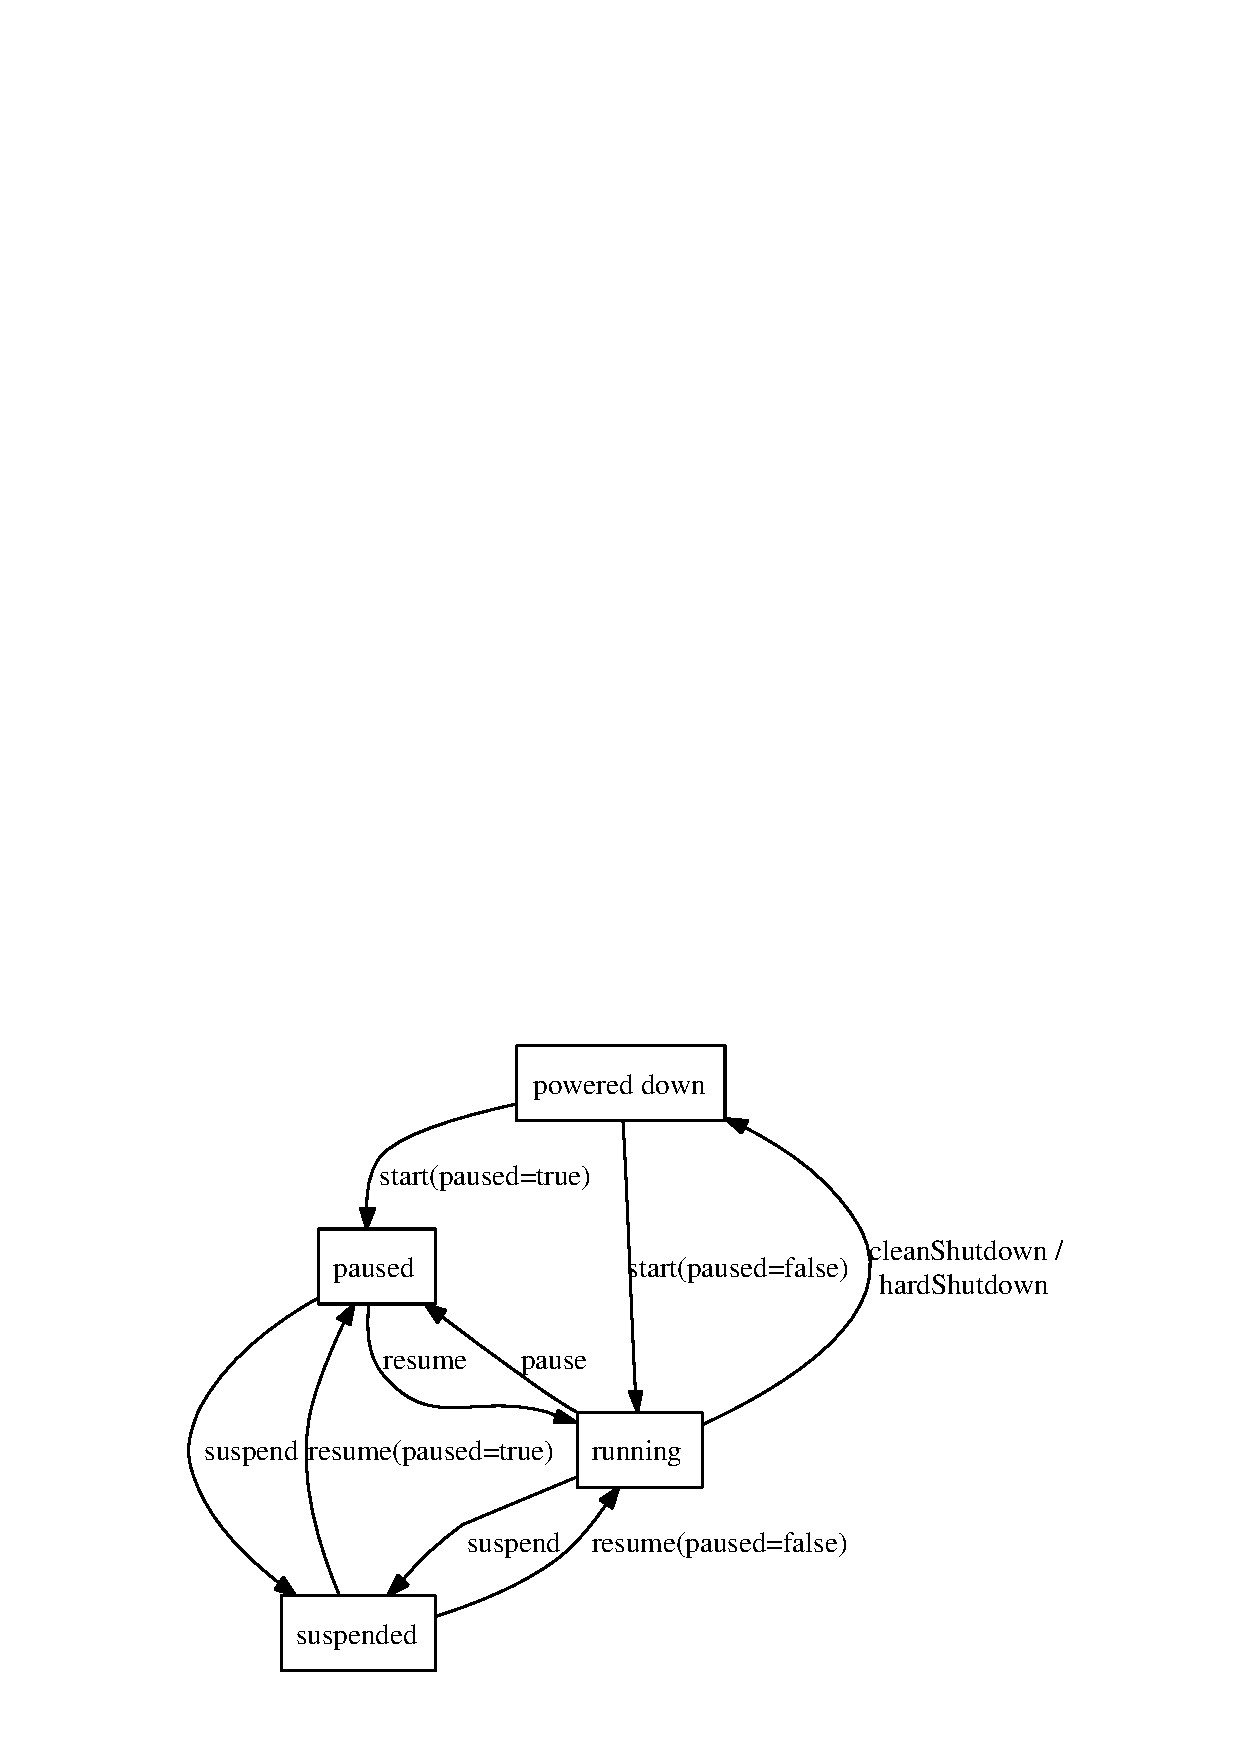
\includegraphics{vm_lifecycle}}
\caption{VM Lifecycle}
\label{fig-vm-lifecycle}
\end{figure}

Figure~\ref{fig-vm-lifecycle} shows the states that a VM can be in
and the API calls that can be used to move the VM between these states.

\section{VM boot parameters}

The VM class contains a number of fields that control the way in which the VM is booted.
With reference to the fields defined in the VM class (see later in this document),
this section outlines the boot options available and the mechanisms provided for controlling them.

VM booting is controlled by setting one of the two mutually exclusive groups: ``PV'', and ``HVM''.  If HVM.boot\_policy is the empty string, then paravirtual domain building and booting will be used; otherwise the VM will be loaded as an HVM domain, and booted using an emulated BIOS.

When paravirtual booting is in use, the PV/bootloader field indicates the bootloader to use.  It may be ``pygrub'', in which case the platform's default installation of pygrub will be used, or a full path within the control domain to some other bootloader.  The other fields, PV/kernel, PV/ramdisk, PV/args and PV/bootloader\_args will be passed to the bootloader unmodified, and interpretation of those fields is then specific to the bootloader itself, including the possibility that the bootloader will ignore some or all of those given values. Finally the paths of all bootable disks are added to the bootloader commandline (a disk is bootable if its VBD has the bootable flag set). There may be zero, one or many bootable disks; the bootloader decides which disk (if any) to boot from.

If the bootloader is pygrub, then the menu.lst is parsed if present in the guest's filesystem, otherwise the specified kernel and ramdisk are used, or an autodetected kernel is used if nothing is specified and autodetection is possible.  PV/args is appended to the kernel command line, no matter which mechanism is used for finding the kernel.

If PV/bootloader is empty but PV/kernel is specified, then the kernel and ramdisk values will be treated as paths within the control domain.  If both PV/bootloader and PV/kernel are empty, then the behaviour is as if PV/bootloader was specified as ``pygrub''.

When using HVM booting, HVM/boot\_policy and HVM/boot\_params specify the boot handling.  Only one policy is currently defined: ``BIOS order''.  In this case, HVM/boot\_params should contain one key-value pair ``order'' = ``N'' where N is the string that will be passed to QEMU.
\include{xenapi-datamodel}
\chapter{GNU Free Documentation License}
%\label{label_fdl}

 \begin{center}

       Version 1.2, November 2002


 Copyright \copyright 2000,2001,2002  Free Software Foundation, Inc.
 
 \bigskip
 
     51 Franklin St, Fifth Floor, Boston, MA  02110-1301  USA
  
 \bigskip
 
 Everyone is permitted to copy and distribute verbatim copies
 of this license document, but changing it is not allowed.
\end{center}


\begin{center}
{\bf\large Preamble}
\end{center}

The purpose of this License is to make a manual, textbook, or other
functional and useful document "free" in the sense of freedom: to
assure everyone the effective freedom to copy and redistribute it,
with or without modifying it, either commercially or noncommercially.
Secondarily, this License preserves for the author and publisher a way
to get credit for their work, while not being considered responsible
for modifications made by others.

This License is a kind of "copyleft", which means that derivative
works of the document must themselves be free in the same sense.  It
complements the GNU General Public License, which is a copyleft
license designed for free software.

We have designed this License in order to use it for manuals for free
software, because free software needs free documentation: a free
program should come with manuals providing the same freedoms that the
software does.  But this License is not limited to software manuals;
it can be used for any textual work, regardless of subject matter or
whether it is published as a printed book.  We recommend this License
principally for works whose purpose is instruction or reference.


\begin{center}
{\Large\bf 1. APPLICABILITY AND DEFINITIONS}
\addcontentsline{toc}{section}{1. APPLICABILITY AND DEFINITIONS}
\end{center}

This License applies to any manual or other work, in any medium, that
contains a notice placed by the copyright holder saying it can be
distributed under the terms of this License.  Such a notice grants a
world-wide, royalty-free license, unlimited in duration, to use that
work under the conditions stated herein.  The \textbf{"Document"}, below,
refers to any such manual or work.  Any member of the public is a
licensee, and is addressed as \textbf{"you"}.  You accept the license if you
copy, modify or distribute the work in a way requiring permission
under copyright law.

A \textbf{"Modified Version"} of the Document means any work containing the
Document or a portion of it, either copied verbatim, or with
modifications and/or translated into another language.

A \textbf{"Secondary Section"} is a named appendix or a front-matter section of
the Document that deals exclusively with the relationship of the
publishers or authors of the Document to the Document's overall subject
(or to related matters) and contains nothing that could fall directly
within that overall subject.  (Thus, if the Document is in part a
textbook of mathematics, a Secondary Section may not explain any
mathematics.)  The relationship could be a matter of historical
connection with the subject or with related matters, or of legal,
commercial, philosophical, ethical or political position regarding
them.

The \textbf{"Invariant Sections"} are certain Secondary Sections whose titles
are designated, as being those of Invariant Sections, in the notice
that says that the Document is released under this License.  If a
section does not fit the above definition of Secondary then it is not
allowed to be designated as Invariant.  The Document may contain zero
Invariant Sections.  If the Document does not identify any Invariant
Sections then there are none.

The \textbf{"Cover Texts"} are certain short passages of text that are listed,
as Front-Cover Texts or Back-Cover Texts, in the notice that says that
the Document is released under this License.  A Front-Cover Text may
be at most 5 words, and a Back-Cover Text may be at most 25 words.

A \textbf{"Transparent"} copy of the Document means a machine-readable copy,
represented in a format whose specification is available to the
general public, that is suitable for revising the document
straightforwardly with generic text editors or (for images composed of
pixels) generic paint programs or (for drawings) some widely available
drawing editor, and that is suitable for input to text formatters or
for automatic translation to a variety of formats suitable for input
to text formatters.  A copy made in an otherwise Transparent file
format whose markup, or absence of markup, has been arranged to thwart
or discourage subsequent modification by readers is not Transparent.
An image format is not Transparent if used for any substantial amount
of text.  A copy that is not "Transparent" is called \textbf{"Opaque"}.

Examples of suitable formats for Transparent copies include plain
ASCII without markup, Texinfo input format, LaTeX input format, SGML
or XML using a publicly available DTD, and standard-conforming simple
HTML, PostScript or PDF designed for human modification.  Examples of
transparent image formats include PNG, XCF and JPG.  Opaque formats
include proprietary formats that can be read and edited only by
proprietary word processors, SGML or XML for which the DTD and/or
processing tools are not generally available, and the
machine-generated HTML, PostScript or PDF produced by some word
processors for output purposes only.

The \textbf{"Title Page"} means, for a printed book, the title page itself,
plus such following pages as are needed to hold, legibly, the material
this License requires to appear in the title page.  For works in
formats which do not have any title page as such, "Title Page" means
the text near the most prominent appearance of the work's title,
preceding the beginning of the body of the text.

A section \textbf{"Entitled XYZ"} means a named subunit of the Document whose
title either is precisely XYZ or contains XYZ in parentheses following
text that translates XYZ in another language.  (Here XYZ stands for a
specific section name mentioned below, such as \textbf{"Acknowledgements"},
\textbf{"Dedications"}, \textbf{"Endorsements"}, or \textbf{"History"}.)  
To \textbf{"Preserve the Title"}
of such a section when you modify the Document means that it remains a
section "Entitled XYZ" according to this definition.

The Document may include Warranty Disclaimers next to the notice which
states that this License applies to the Document.  These Warranty
Disclaimers are considered to be included by reference in this
License, but only as regards disclaiming warranties: any other
implication that these Warranty Disclaimers may have is void and has
no effect on the meaning of this License.


\begin{center}
{\Large\bf 2. VERBATIM COPYING}
\addcontentsline{toc}{section}{2. VERBATIM COPYING}
\end{center}

You may copy and distribute the Document in any medium, either
commercially or noncommercially, provided that this License, the
copyright notices, and the license notice saying this License applies
to the Document are reproduced in all copies, and that you add no other
conditions whatsoever to those of this License.  You may not use
technical measures to obstruct or control the reading or further
copying of the copies you make or distribute.  However, you may accept
compensation in exchange for copies.  If you distribute a large enough
number of copies you must also follow the conditions in section 3.

You may also lend copies, under the same conditions stated above, and
you may publicly display copies.


\begin{center}
{\Large\bf 3. COPYING IN QUANTITY}
\addcontentsline{toc}{section}{3. COPYING IN QUANTITY}
\end{center}


If you publish printed copies (or copies in media that commonly have
printed covers) of the Document, numbering more than 100, and the
Document's license notice requires Cover Texts, you must enclose the
copies in covers that carry, clearly and legibly, all these Cover
Texts: Front-Cover Texts on the front cover, and Back-Cover Texts on
the back cover.  Both covers must also clearly and legibly identify
you as the publisher of these copies.  The front cover must present
the full title with all words of the title equally prominent and
visible.  You may add other material on the covers in addition.
Copying with changes limited to the covers, as long as they preserve
the title of the Document and satisfy these conditions, can be treated
as verbatim copying in other respects.

If the required texts for either cover are too voluminous to fit
legibly, you should put the first ones listed (as many as fit
reasonably) on the actual cover, and continue the rest onto adjacent
pages.

If you publish or distribute Opaque copies of the Document numbering
more than 100, you must either include a machine-readable Transparent
copy along with each Opaque copy, or state in or with each Opaque copy
a computer-network location from which the general network-using
public has access to download using public-standard network protocols
a complete Transparent copy of the Document, free of added material.
If you use the latter option, you must take reasonably prudent steps,
when you begin distribution of Opaque copies in quantity, to ensure
that this Transparent copy will remain thus accessible at the stated
location until at least one year after the last time you distribute an
Opaque copy (directly or through your agents or retailers) of that
edition to the public.

It is requested, but not required, that you contact the authors of the
Document well before redistributing any large number of copies, to give
them a chance to provide you with an updated version of the Document.


\begin{center}
{\Large\bf 4. MODIFICATIONS}
\addcontentsline{toc}{section}{4. MODIFICATIONS}
\end{center}

You may copy and distribute a Modified Version of the Document under
the conditions of sections 2 and 3 above, provided that you release
the Modified Version under precisely this License, with the Modified
Version filling the role of the Document, thus licensing distribution
and modification of the Modified Version to whoever possesses a copy
of it.  In addition, you must do these things in the Modified Version:

\begin{itemize}
\item[A.] 
   Use in the Title Page (and on the covers, if any) a title distinct
   from that of the Document, and from those of previous versions
   (which should, if there were any, be listed in the History section
   of the Document).  You may use the same title as a previous version
   if the original publisher of that version gives permission.
   
\item[B.]
   List on the Title Page, as authors, one or more persons or entities
   responsible for authorship of the modifications in the Modified
   Version, together with at least five of the principal authors of the
   Document (all of its principal authors, if it has fewer than five),
   unless they release you from this requirement.
   
\item[C.]
   State on the Title page the name of the publisher of the
   Modified Version, as the publisher.
   
\item[D.]
   Preserve all the copyright notices of the Document.
   
\item[E.]
   Add an appropriate copyright notice for your modifications
   adjacent to the other copyright notices.
   
\item[F.]
   Include, immediately after the copyright notices, a license notice
   giving the public permission to use the Modified Version under the
   terms of this License, in the form shown in the Addendum below.
   
\item[G.]
   Preserve in that license notice the full lists of Invariant Sections
   and required Cover Texts given in the Document's license notice.
   
\item[H.]
   Include an unaltered copy of this License.
   
\item[I.]
   Preserve the section Entitled "History", Preserve its Title, and add
   to it an item stating at least the title, year, new authors, and
   publisher of the Modified Version as given on the Title Page.  If
   there is no section Entitled "History" in the Document, create one
   stating the title, year, authors, and publisher of the Document as
   given on its Title Page, then add an item describing the Modified
   Version as stated in the previous sentence.
   
\item[J.]
   Preserve the network location, if any, given in the Document for
   public access to a Transparent copy of the Document, and likewise
   the network locations given in the Document for previous versions
   it was based on.  These may be placed in the "History" section.
   You may omit a network location for a work that was published at
   least four years before the Document itself, or if the original
   publisher of the version it refers to gives permission.
   
\item[K.]
   For any section Entitled "Acknowledgements" or "Dedications",
   Preserve the Title of the section, and preserve in the section all
   the substance and tone of each of the contributor acknowledgements
   and/or dedications given therein.
   
\item[L.]
   Preserve all the Invariant Sections of the Document,
   unaltered in their text and in their titles.  Section numbers
   or the equivalent are not considered part of the section titles.
   
\item[M.]
   Delete any section Entitled "Endorsements".  Such a section
   may not be included in the Modified Version.
   
\item[N.]
   Do not retitle any existing section to be Entitled "Endorsements"
   or to conflict in title with any Invariant Section.
   
\item[O.]
   Preserve any Warranty Disclaimers.
\end{itemize}

If the Modified Version includes new front-matter sections or
appendices that qualify as Secondary Sections and contain no material
copied from the Document, you may at your option designate some or all
of these sections as invariant.  To do this, add their titles to the
list of Invariant Sections in the Modified Version's license notice.
These titles must be distinct from any other section titles.

You may add a section Entitled "Endorsements", provided it contains
nothing but endorsements of your Modified Version by various
parties--for example, statements of peer review or that the text has
been approved by an organization as the authoritative definition of a
standard.

You may add a passage of up to five words as a Front-Cover Text, and a
passage of up to 25 words as a Back-Cover Text, to the end of the list
of Cover Texts in the Modified Version.  Only one passage of
Front-Cover Text and one of Back-Cover Text may be added by (or
through arrangements made by) any one entity.  If the Document already
includes a cover text for the same cover, previously added by you or
by arrangement made by the same entity you are acting on behalf of,
you may not add another; but you may replace the old one, on explicit
permission from the previous publisher that added the old one.

The author(s) and publisher(s) of the Document do not by this License
give permission to use their names for publicity for or to assert or
imply endorsement of any Modified Version.


\begin{center}
{\Large\bf 5. COMBINING DOCUMENTS}
\addcontentsline{toc}{section}{5. COMBINING DOCUMENTS}
\end{center}


You may combine the Document with other documents released under this
License, under the terms defined in section 4 above for modified
versions, provided that you include in the combination all of the
Invariant Sections of all of the original documents, unmodified, and
list them all as Invariant Sections of your combined work in its
license notice, and that you preserve all their Warranty Disclaimers.

The combined work need only contain one copy of this License, and
multiple identical Invariant Sections may be replaced with a single
copy.  If there are multiple Invariant Sections with the same name but
different contents, make the title of each such section unique by
adding at the end of it, in parentheses, the name of the original
author or publisher of that section if known, or else a unique number.
Make the same adjustment to the section titles in the list of
Invariant Sections in the license notice of the combined work.

In the combination, you must combine any sections Entitled "History"
in the various original documents, forming one section Entitled
"History"; likewise combine any sections Entitled "Acknowledgements",
and any sections Entitled "Dedications".  You must delete all sections
Entitled "Endorsements".

\begin{center}
{\Large\bf 6. COLLECTIONS OF DOCUMENTS}
\addcontentsline{toc}{section}{6. COLLECTIONS OF DOCUMENTS}
\end{center}

You may make a collection consisting of the Document and other documents
released under this License, and replace the individual copies of this
License in the various documents with a single copy that is included in
the collection, provided that you follow the rules of this License for
verbatim copying of each of the documents in all other respects.

You may extract a single document from such a collection, and distribute
it individually under this License, provided you insert a copy of this
License into the extracted document, and follow this License in all
other respects regarding verbatim copying of that document.


\begin{center}
{\Large\bf 7. AGGREGATION WITH INDEPENDENT WORKS}
\addcontentsline{toc}{section}{7. AGGREGATION WITH INDEPENDENT WORKS}
\end{center}


A compilation of the Document or its derivatives with other separate
and independent documents or works, in or on a volume of a storage or
distribution medium, is called an "aggregate" if the copyright
resulting from the compilation is not used to limit the legal rights
of the compilation's users beyond what the individual works permit.
When the Document is included in an aggregate, this License does not
apply to the other works in the aggregate which are not themselves
derivative works of the Document.

If the Cover Text requirement of section 3 is applicable to these
copies of the Document, then if the Document is less than one half of
the entire aggregate, the Document's Cover Texts may be placed on
covers that bracket the Document within the aggregate, or the
electronic equivalent of covers if the Document is in electronic form.
Otherwise they must appear on printed covers that bracket the whole
aggregate.


\begin{center}
{\Large\bf 8. TRANSLATION}
\addcontentsline{toc}{section}{8. TRANSLATION}
\end{center}


Translation is considered a kind of modification, so you may
distribute translations of the Document under the terms of section 4.
Replacing Invariant Sections with translations requires special
permission from their copyright holders, but you may include
translations of some or all Invariant Sections in addition to the
original versions of these Invariant Sections.  You may include a
translation of this License, and all the license notices in the
Document, and any Warranty Disclaimers, provided that you also include
the original English version of this License and the original versions
of those notices and disclaimers.  In case of a disagreement between
the translation and the original version of this License or a notice
or disclaimer, the original version will prevail.

If a section in the Document is Entitled "Acknowledgements",
"Dedications", or "History", the requirement (section 4) to Preserve
its Title (section 1) will typically require changing the actual
title.


\begin{center}
{\Large\bf 9. TERMINATION}
\addcontentsline{toc}{section}{9. TERMINATION}
\end{center}


You may not copy, modify, sublicense, or distribute the Document except
as expressly provided for under this License.  Any other attempt to
copy, modify, sublicense or distribute the Document is void, and will
automatically terminate your rights under this License.  However,
parties who have received copies, or rights, from you under this
License will not have their licenses terminated so long as such
parties remain in full compliance.


\begin{center}
{\Large\bf 10. FUTURE REVISIONS OF THIS LICENSE}
\addcontentsline{toc}{section}{10. FUTURE REVISIONS OF THIS LICENSE}
\end{center}


The Free Software Foundation may publish new, revised versions
of the GNU Free Documentation License from time to time.  Such new
versions will be similar in spirit to the present version, but may
differ in detail to address new problems or concerns.  See
http://www.gnu.org/copyleft/.

Each version of the License is given a distinguishing version number.
If the Document specifies that a particular numbered version of this
License "or any later version" applies to it, you have the option of
following the terms and conditions either of that specified version or
of any later version that has been published (not as a draft) by the
Free Software Foundation.  If the Document does not specify a version
number of this License, you may choose any version ever published (not
as a draft) by the Free Software Foundation.


\begin{center}
{\Large\bf ADDENDUM: How to use this License for your documents}
\addcontentsline{toc}{section}{ADDENDUM: How to use this License for your documents}
\end{center}

To use this License in a document you have written, include a copy of
the License in the document and put the following copyright and
license notices just after the title page:

\bigskip
\begin{quote}
    Copyright \copyright  YEAR  YOUR NAME.
    Permission is granted to copy, distribute and/or modify this document
    under the terms of the GNU Free Documentation License, Version 1.2
    or any later version published by the Free Software Foundation;
    with no Invariant Sections, no Front-Cover Texts, and no Back-Cover Texts.
    A copy of the license is included in the section entitled "GNU
    Free Documentation License".
\end{quote}
\bigskip
    
If you have Invariant Sections, Front-Cover Texts and Back-Cover Texts,
replace the "with...Texts." line with this:

\bigskip
\begin{quote}
    with the Invariant Sections being LIST THEIR TITLES, with the
    Front-Cover Texts being LIST, and with the Back-Cover Texts being LIST.
\end{quote}
\bigskip
    
If you have Invariant Sections without Cover Texts, or some other
combination of the three, merge those two alternatives to suit the
situation.

If your document contains nontrivial examples of program code, we
recommend releasing these examples in parallel under your choice of
free software license, such as the GNU General Public License,
to permit their use in free software.


\end{document}
